\hypertarget{openmote-cc2538_2lwip_2src_2include_2lwip_2etharp_8h}{}\section{/home/ayush/\+R\+I\+O\+T/tests/lwip/bin/pkg/openmote-\/cc2538/lwip/src/include/lwip/etharp.h File Reference}
\label{openmote-cc2538_2lwip_2src_2include_2lwip_2etharp_8h}\index{/home/ayush/\+R\+I\+O\+T/tests/lwip/bin/pkg/openmote-\/cc2538/lwip/src/include/lwip/etharp.\+h@{/home/ayush/\+R\+I\+O\+T/tests/lwip/bin/pkg/openmote-\/cc2538/lwip/src/include/lwip/etharp.\+h}}
{\ttfamily \#include \char`\"{}lwip/opt.\+h\char`\"{}}\newline
Include dependency graph for etharp.\+h\+:
\nopagebreak
\begin{figure}[H]
\begin{center}
\leavevmode
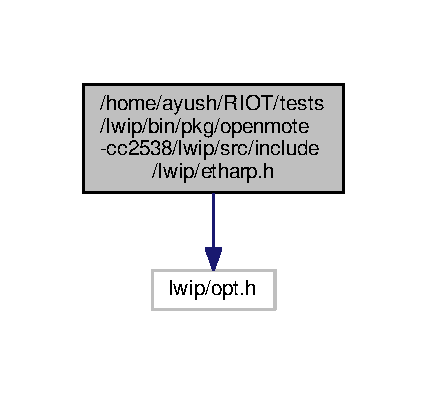
\includegraphics[width=205pt]{openmote-cc2538_2lwip_2src_2include_2lwip_2etharp_8h__incl}
\end{center}
\end{figure}
This graph shows which files directly or indirectly include this file\+:
\nopagebreak
\begin{figure}[H]
\begin{center}
\leavevmode
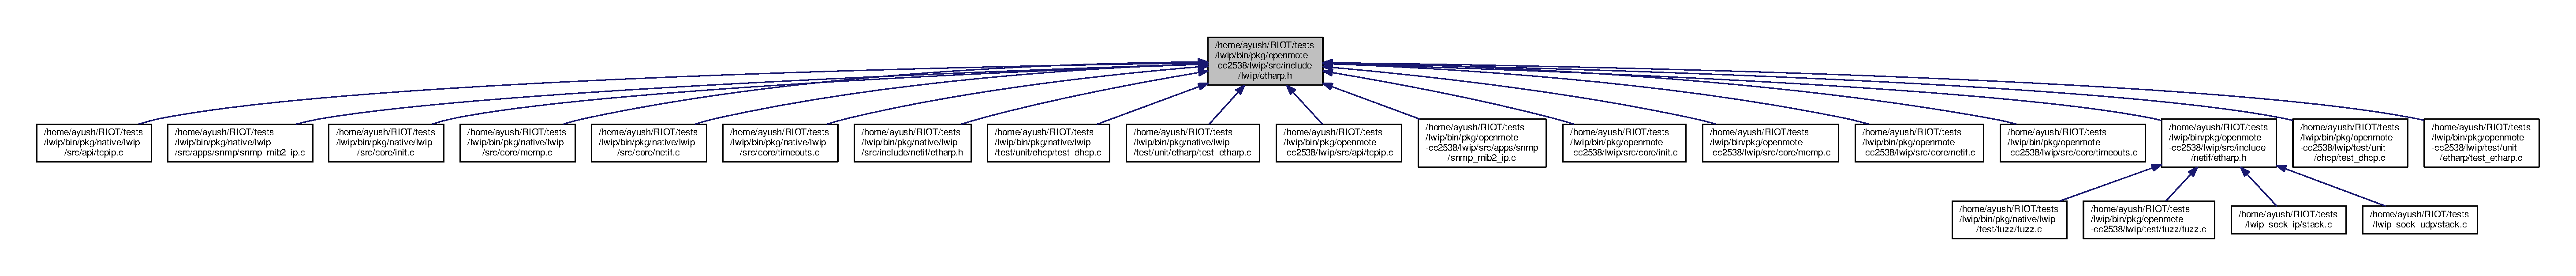
\includegraphics[width=350pt]{openmote-cc2538_2lwip_2src_2include_2lwip_2etharp_8h__dep__incl}
\end{center}
\end{figure}


\subsection{Detailed Description}
Ethernet output function -\/ handles O\+U\+T\+G\+O\+I\+NG ethernet level traffic, implements A\+RP resolving. To be used in most low-\/level netif implementations 